\begin{figure}[H]
    \centering
    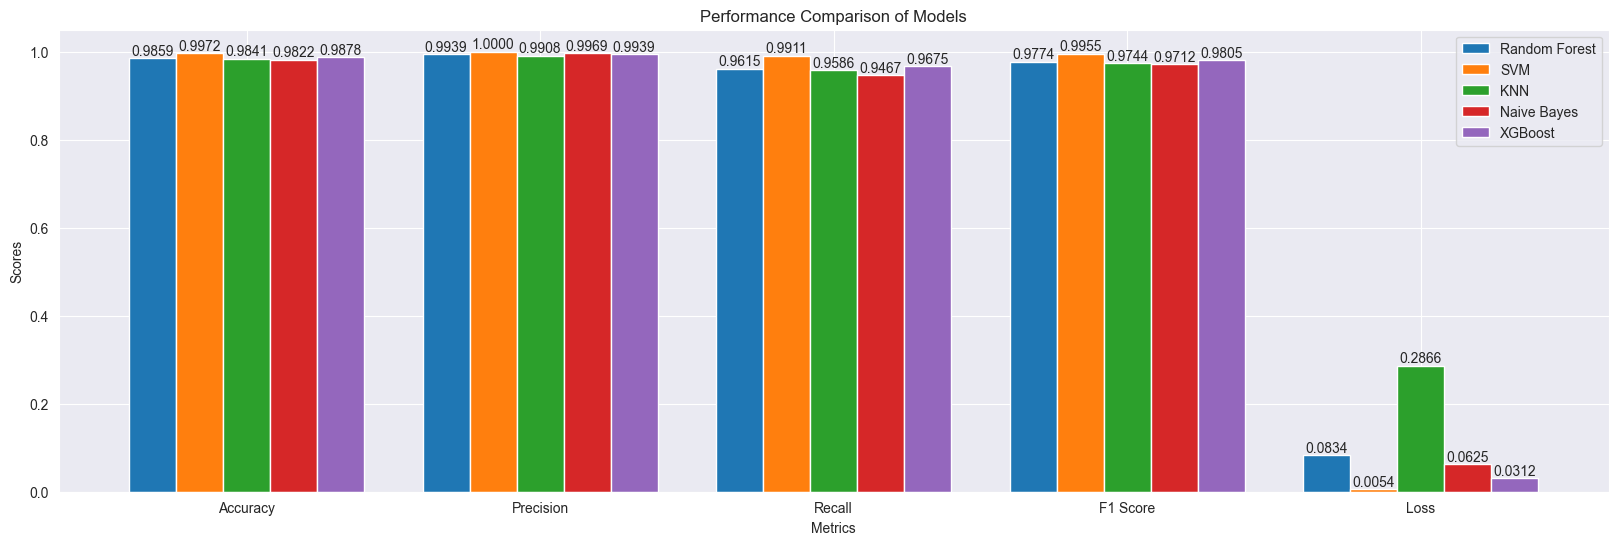
\includegraphics[width=\linewidth]{images/models_performance_train}
    \caption{Comparison of Models' Performance on Training Dataset}
    \label{fig:models_performance_train}
\end{figure}

\begin{itemize}
    \item \textbf{Accuracy:}
    \begin{itemize}
        \item SVM exhibits the highest accuracy (0.9972).
        \item KNN (0.9841), Random Forest (0.9859), Naive Bayes (0.9822), and XGBoost (0.9878) show very competitive and high accuracy scores, all above 0.98.
    \end{itemize}

    \item \textbf{Precision:}
    \begin{itemize}
        \item SVM achieves perfect precision (1.0000).
        \item Random Forest (0.9939), KNN (0.9908), Naive Bayes (0.9969), and XGBoost (0.9939) also demonstrate exceptionally high precision, all above 0.99.
    \end{itemize}

    \item \textbf{Recall:}
    \begin{itemize}
        \item SVM shows the highest recall (0.9911).
        \item XGBoost (0.9675) and Random Forest (0.9615) follow with high recall scores.
        \item KNN (0.9586) and Naive Bayes (0.9467) have slightly lower recall compared to the others, but still maintain strong performance.
    \end{itemize}

    \item \textbf{F1 Score:}
    \begin{itemize}
        \item SVM leads with the highest F1 Score (0.9955).
        \item XGBoost (0.9805) and Random Forest (0.9774) also have excellent F1 Scores, indicating a good balance between precision and recall.
        \item KNN (0.9744) and Naive Bayes (0.9712) show robust F1 Scores as well.
    \end{itemize}

    \item \textbf{Loss:}
    \begin{itemize}
        \item SVM has the lowest loss value (0.0054), indicating the best model fit according to this metric.
        \item XGBoost (0.0312) and Random Forest (0.0834) also have relatively low loss values.
        \item Naive Bayes (0.0625) has a moderate loss.
        \item KNN exhibits the highest loss among the models (0.2866).
    \end{itemize}

    \item \textbf{Overall Observations from the Chart:}
    \begin{itemize}
        \item Across the metrics of Accuracy, Precision, Recall, and F1 Score, SVM consistently performs as the top model or among the top performers.
        \item All models demonstrate very high performance (scores generally $>$ 0.94) for Accuracy, Precision, Recall, and F1 Score, suggesting the effectiveness of the underlying task.
        \item In terms of Loss (where lower is better), SVM is distinctly superior, followed by XGBoost.
        KNN shows a significantly higher loss compared to the other models.
    \end{itemize}
\end{itemize}

\begin{table}[H]
    \centering
    \caption{Model Performance Comparison (Based on Bar Chart)}
    \setlength{\tabcolsep}{3pt}
    \renewcommand{\arraystretch}{1.2}
    \resizebox{240pt}{!}{
        \begin{tabular}{|p{2.8cm}|p{2.8cm}|}
            \hline
            \textbf{Model} & \textbf{Key Analysis}                                                                      \\
            \hline
            Random Forest  & High overall performance. Excellent precision, strong recall \& F1. Moderate loss.         \\
            \hline
            SVM            & Top performer across all metrics. Perfect precision, highest Acc, Recall, F1. Lowest loss. \\
            \hline
            KNN            & Strong performance, slightly below RF / XGBoost. Highest loss among models.                \\
            \hline
            Naive Bayes    & Very high precision. Recall is the lowest among models, impacting F1 slightly. Low loss.   \\
            \hline
            XGBoost        & Excellent performance, second to SVM overall. Very low loss. Strong recall \& F1.          \\
            \hline
        \end{tabular}
    }
    \label{tab:model_performance_barchart}
\end{table}